\section{Grænseflader}
Dette afsnit beskriver systemets grænseflader og hvordan bruger kan interagere med systemet.

\subsection{Brugergrænseflade}
Brugergrænsefladen består af en webapplikation, hvor bruger kan opsætte nye flyveruter, gemme flyveruter og overvåge drone status. Webapplikationen indeholder en database, som muliggøre arkiv funktioner for bruger. 

\subsection{Webapplikation}
Webapplikationen er grænseflade mellem bruger og den resterende del af systemet. 

På figur \ref{fig:mockup_login} ses login vinduet, som bruger bliver præsenteret for når der ønskes at interagere med systemet. Her vil bruger kunne logge ind og opsætte flyveruter, se gamle ruter og billeder fra tidligere flyvninger.

\vspace{-5pt}
%Login mockup
\begin{figure}[H]
	\centering
	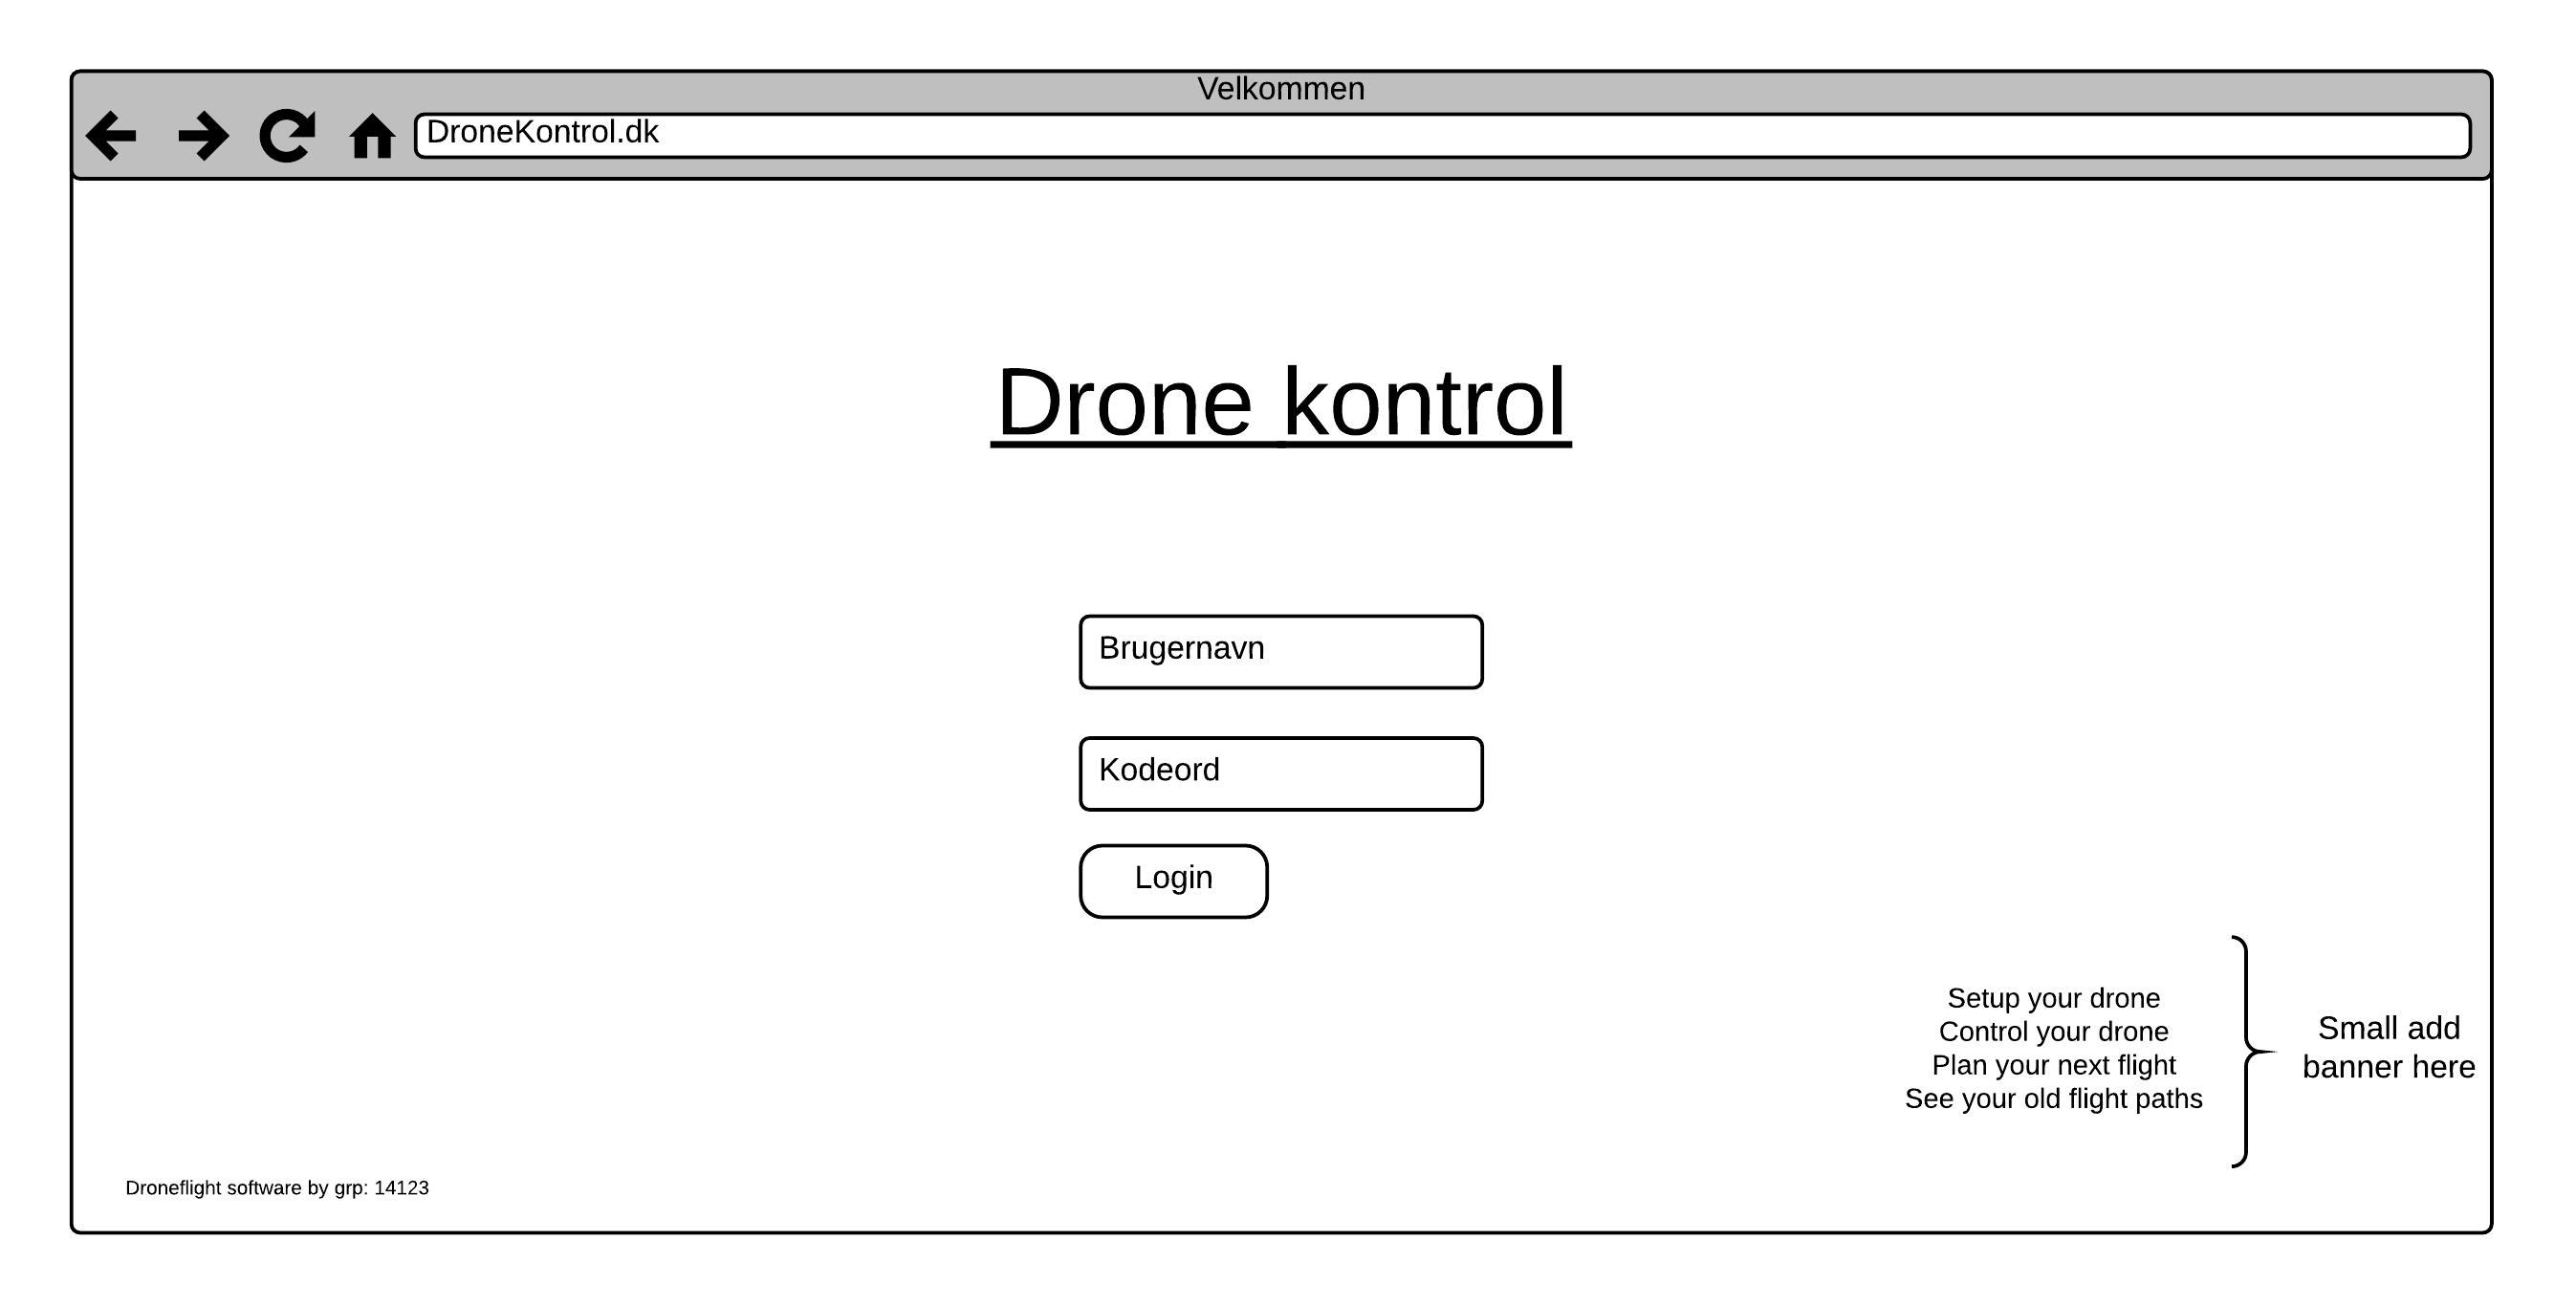
\includegraphics[width=0.9\textwidth]{Billeder/UI_mockups/login.png}
	\vspace{-5pt}
	\caption{Login vindue}
	\label{fig:mockup_login}
\end{figure}

 \newpage

Efter login præsenteres bruger for webapplikations forside, se figur \ref{fig:mockup_welcome}. 
Fra forsiden kan bruger se om der er forbindelse mellem webapplikation og dronen, tilgå Flight bootcamp som er en quick-guiden til flyveopsætning og se en liste med et uddrag af de sidste flyvninger. Øverst på siden kan bruger tilgå opsætning af ny flyvning og den fulde liste med tidligere flyvninger.

\vspace{-5pt}
 %Index mockup
 \begin{figure}[H]
 	\centering
 	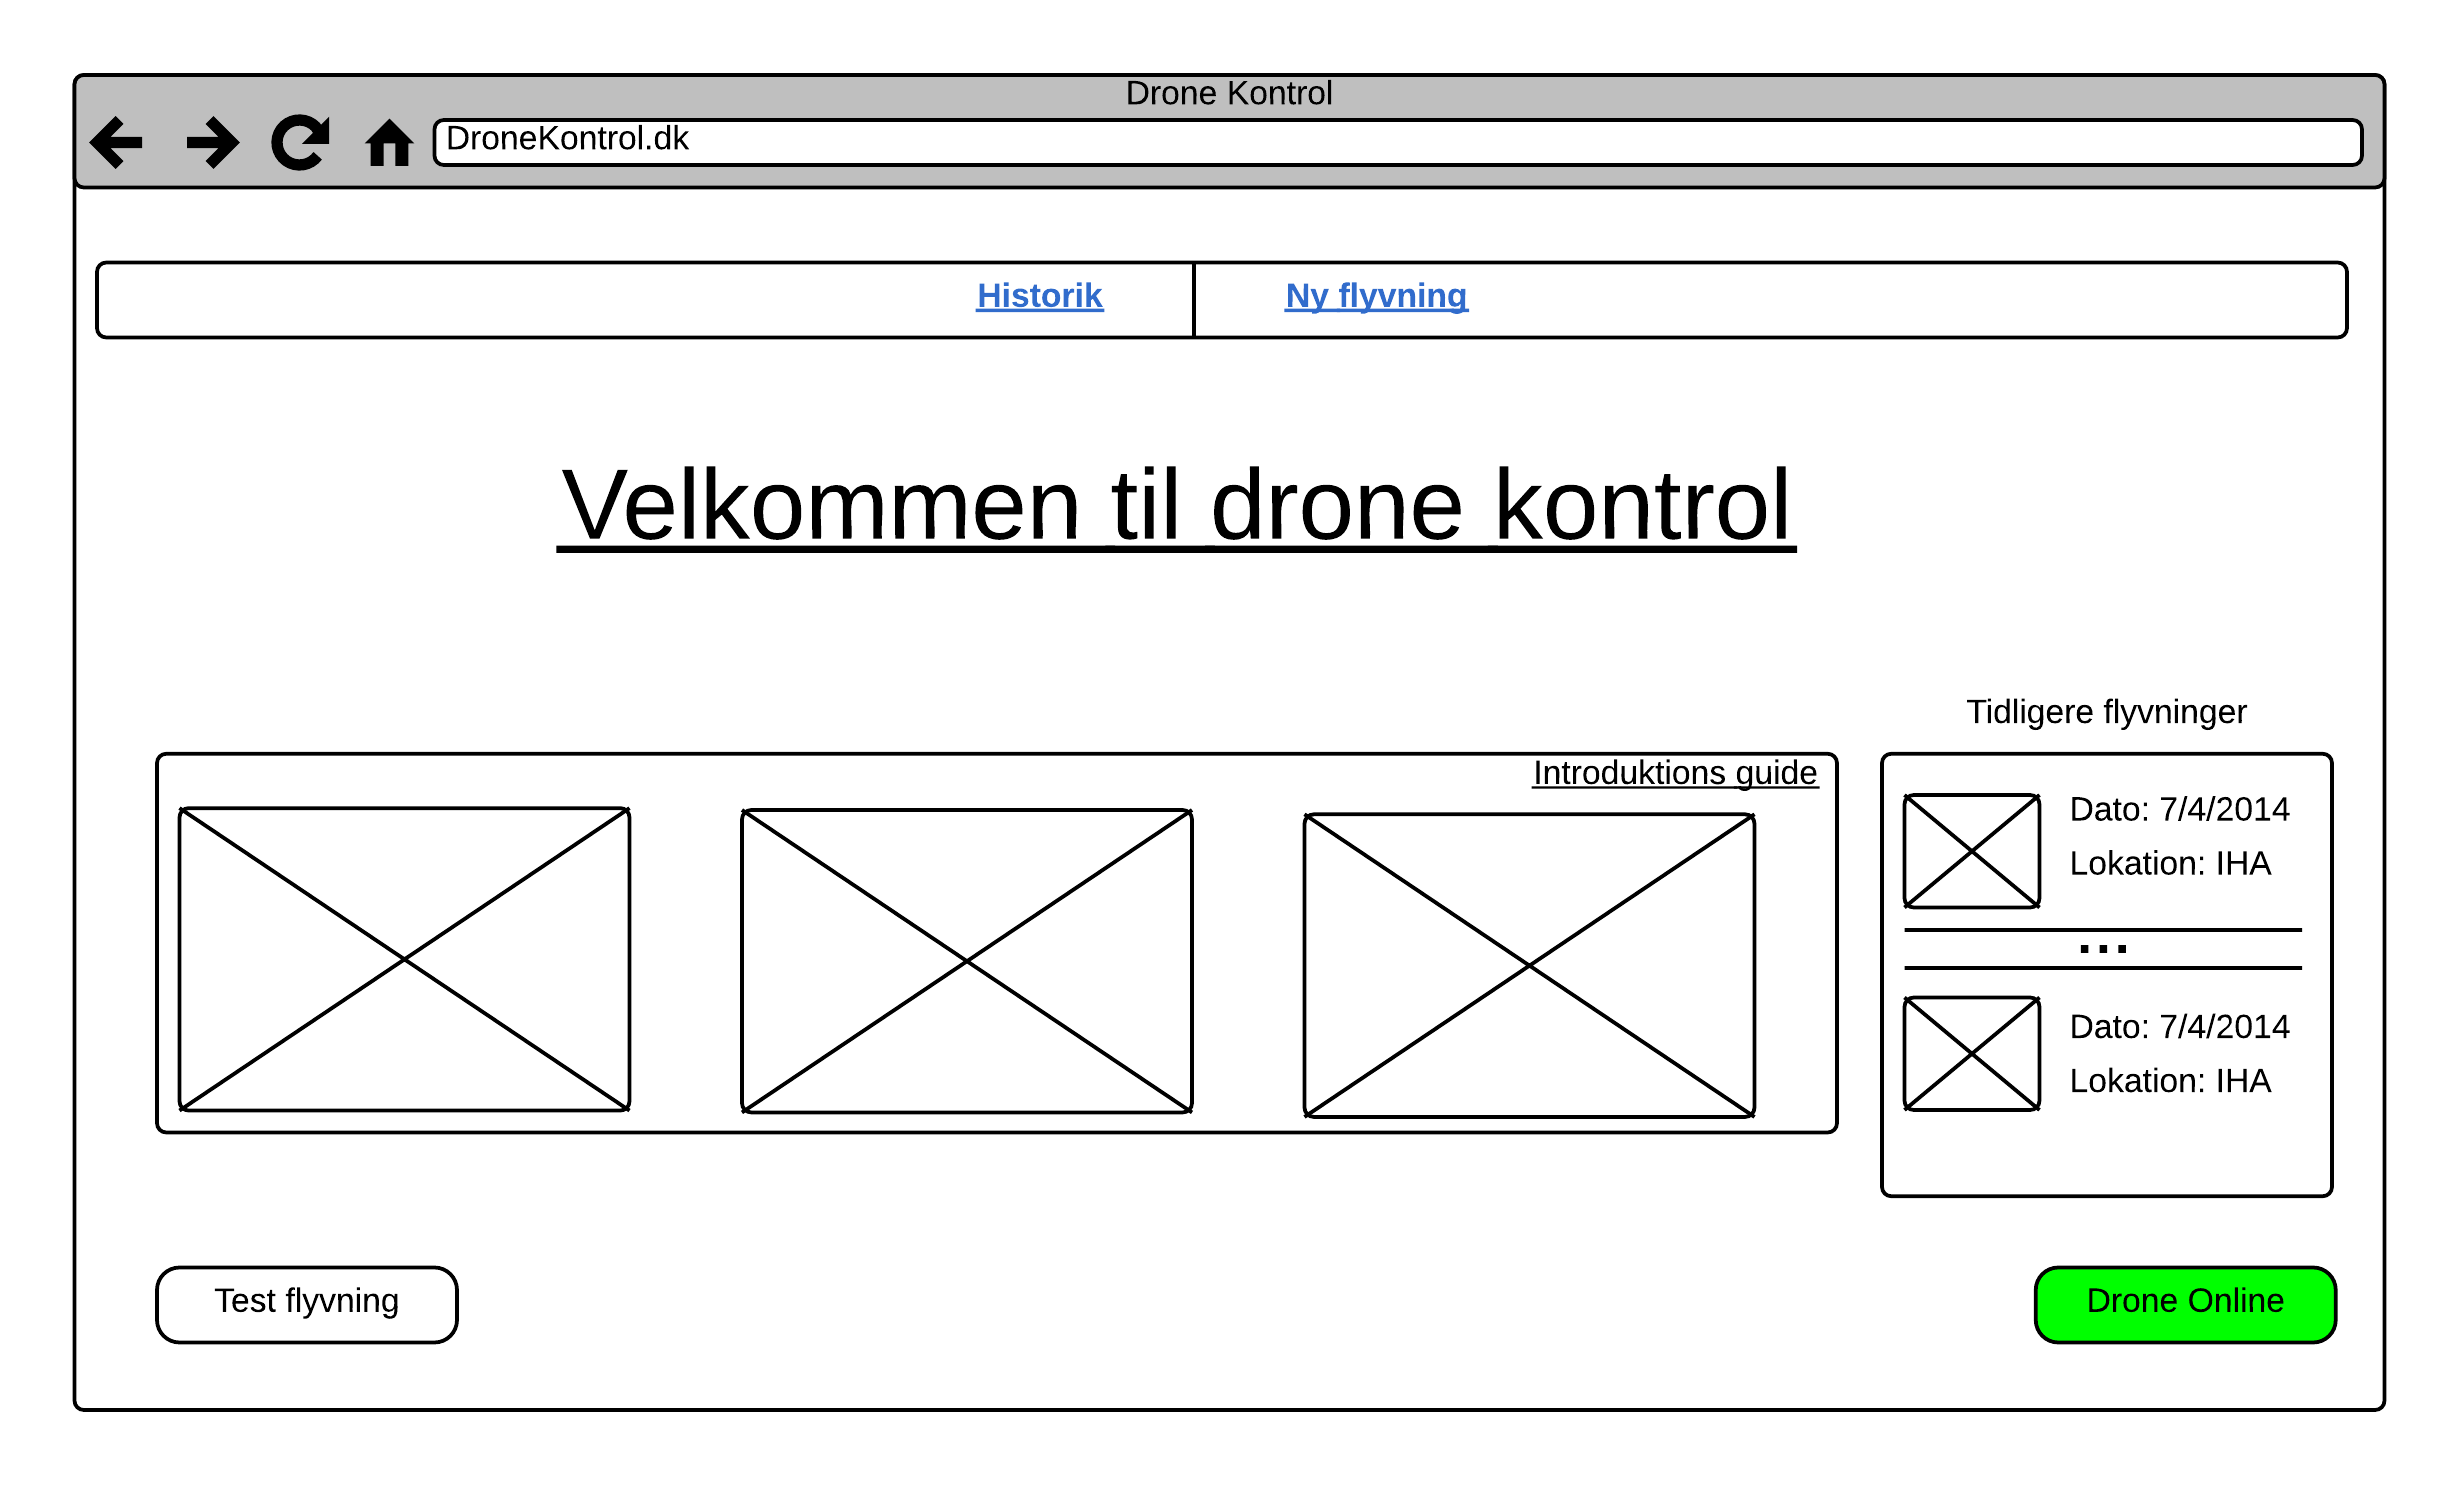
\includegraphics[width=0.9\textwidth]{Billeder/UI_mockups/index.png}
 	\vspace{-5pt}
 	\caption{Velkommen vindue}
 	\label{fig:mockup_welcome}
 \end{figure} 

\vspace{1cm}

I historik menuen har bruger mulighed for at se alle tidligere flyvninger. De tidligere flyvninger præsenteres med hver sin mappe, og mapperne er struktureret efter dato. Da de tidligere flyvninger er struktureret efter dato er det nemt og hurtigt at finde data fra den eller de ønskede flyvninger. Når bruger doubleklikker på en tidligere flyvning åbnes tilhørende mappe, og alt indhold i mappen vises.

\vspace{-5pt}
%Archive mockup
\begin{figure}[H]
	\centering
	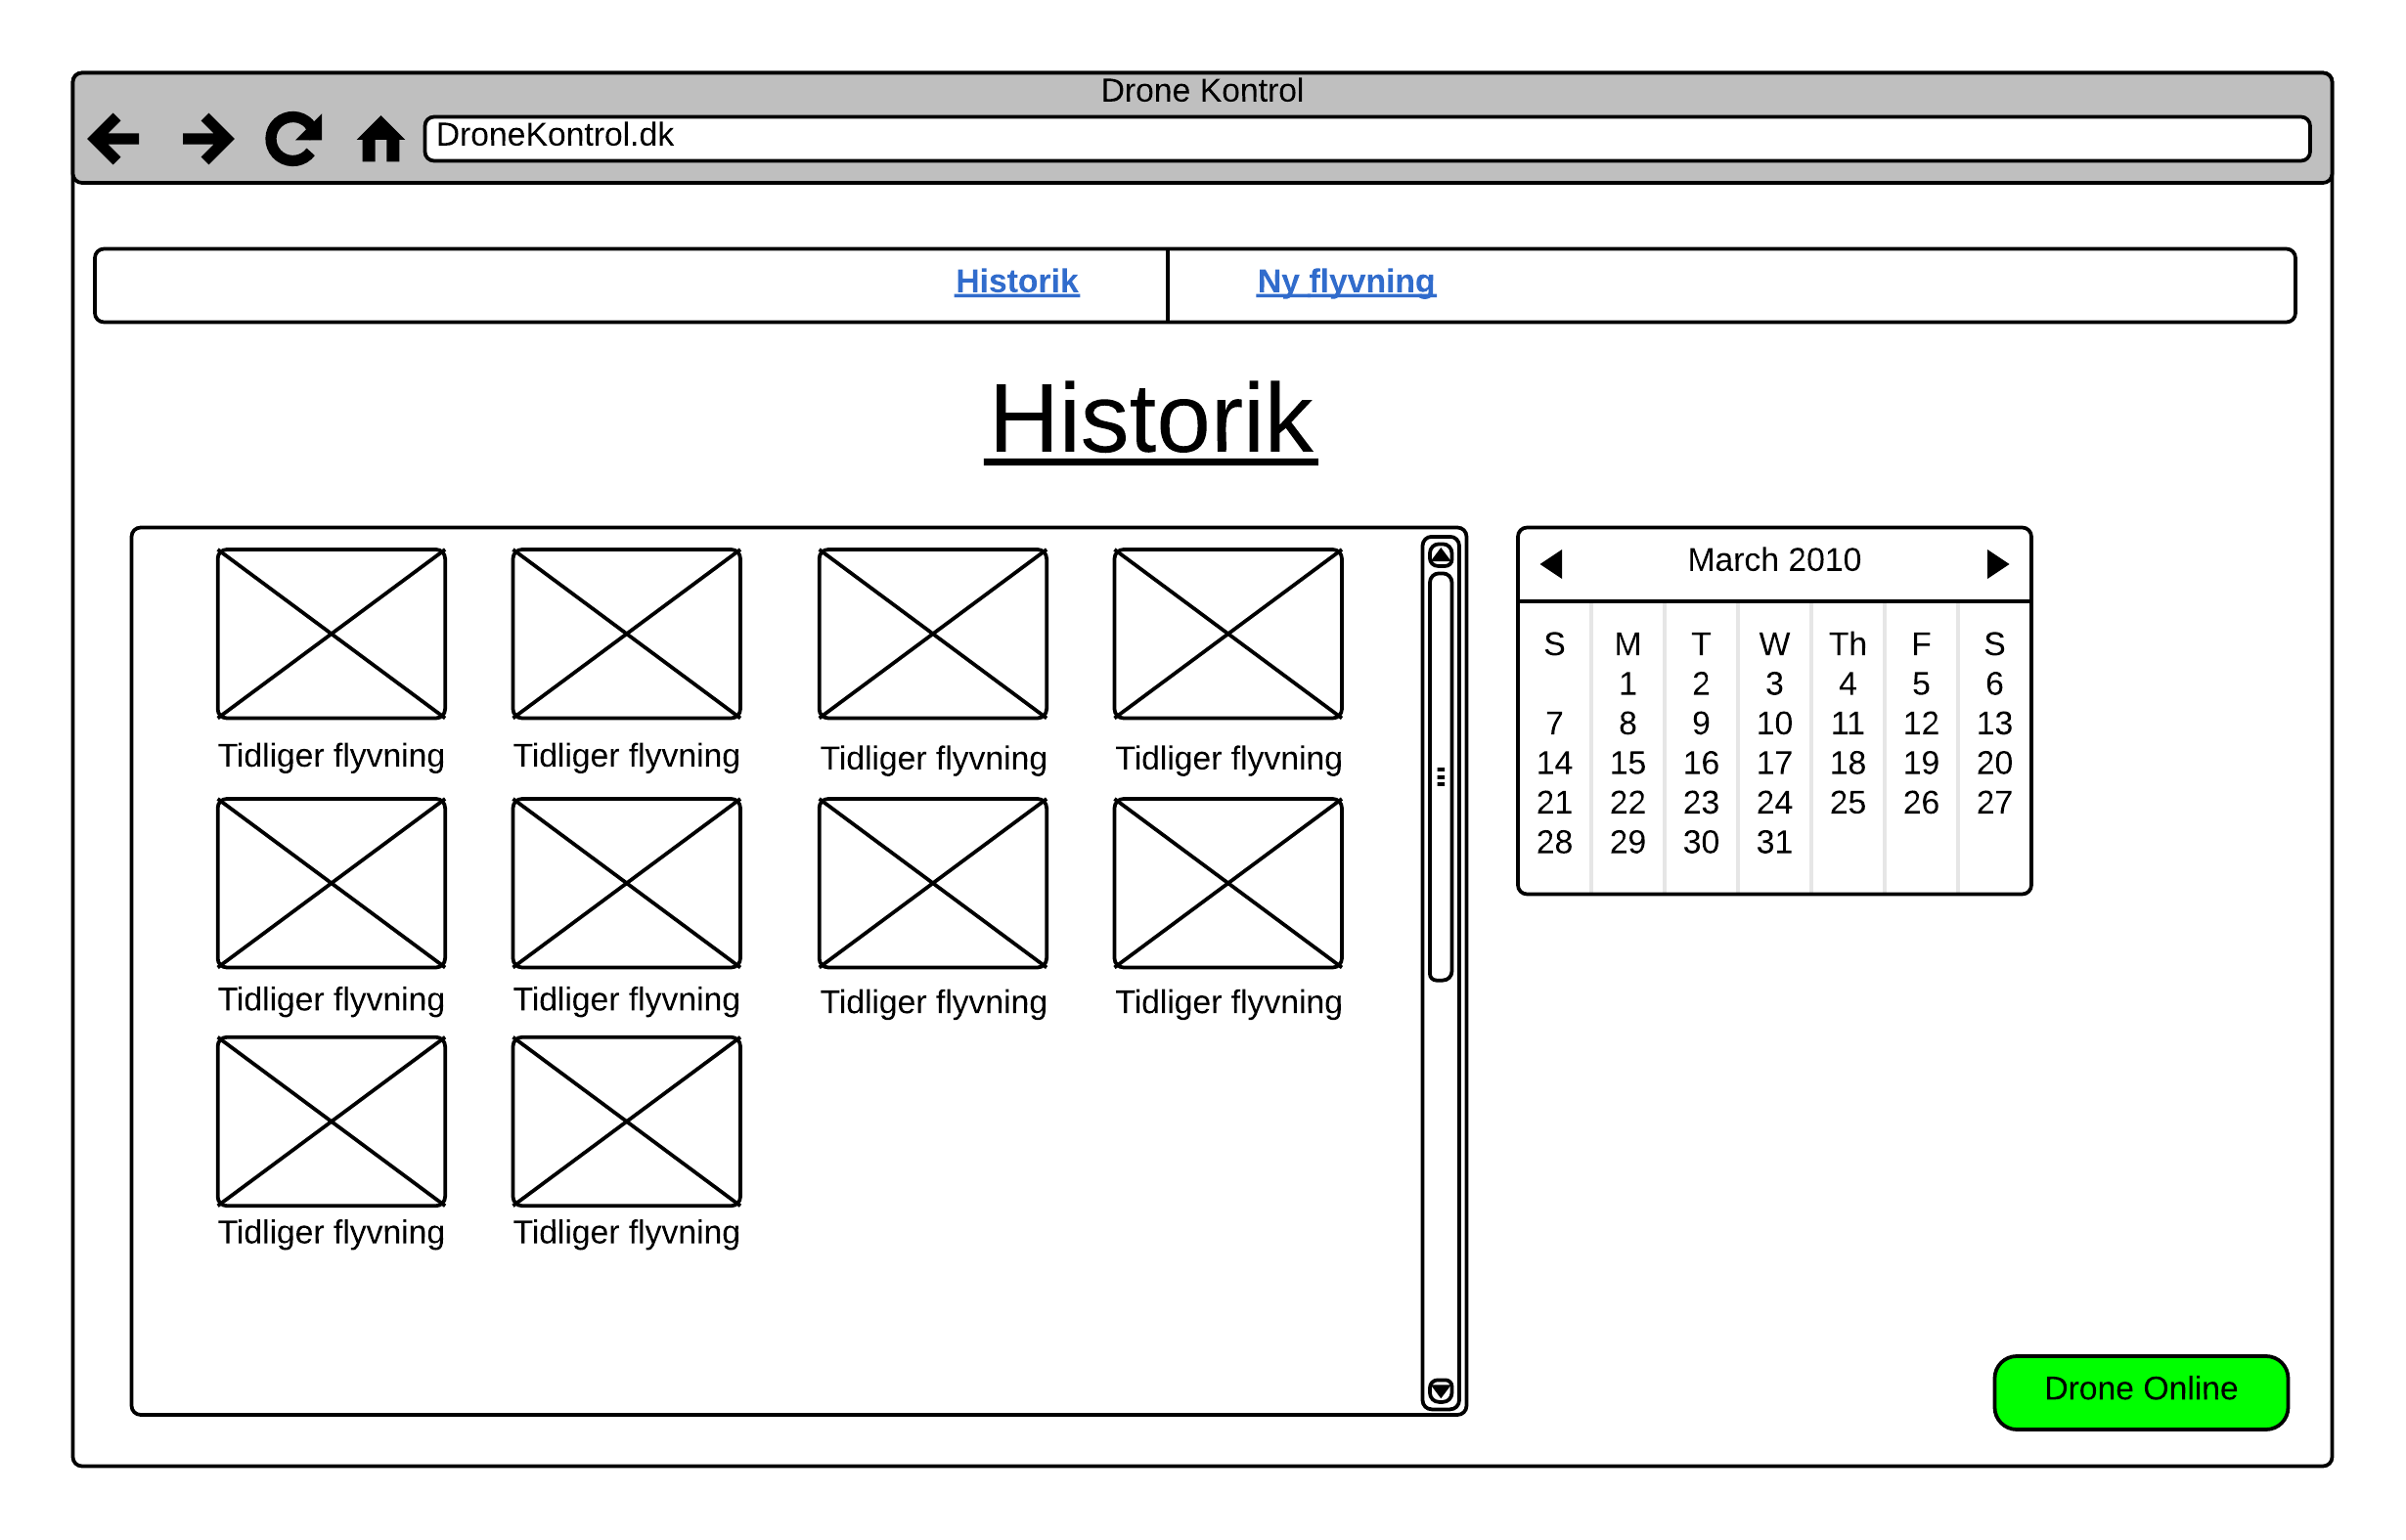
\includegraphics[width=0.9\textwidth]{Billeder/UI_mockups/archive.png}
	\vspace{-5pt}
	\caption{Historik vindue}
	\label{fig:mockup_archive}
\end{figure}

\newpage

Når en tidligere flyvning er valgt, præsenteres bruger for al information tilknyttet den pågældende flyvning. Hvilket betyder bruger får adgang til flyverute, billeder og film sekvenser. På et kort vises den flyveruten dronen gjorde brug af.

\vspace{-5pt}
%Archive choosen mockup
\begin{figure}[H]
	\centering
	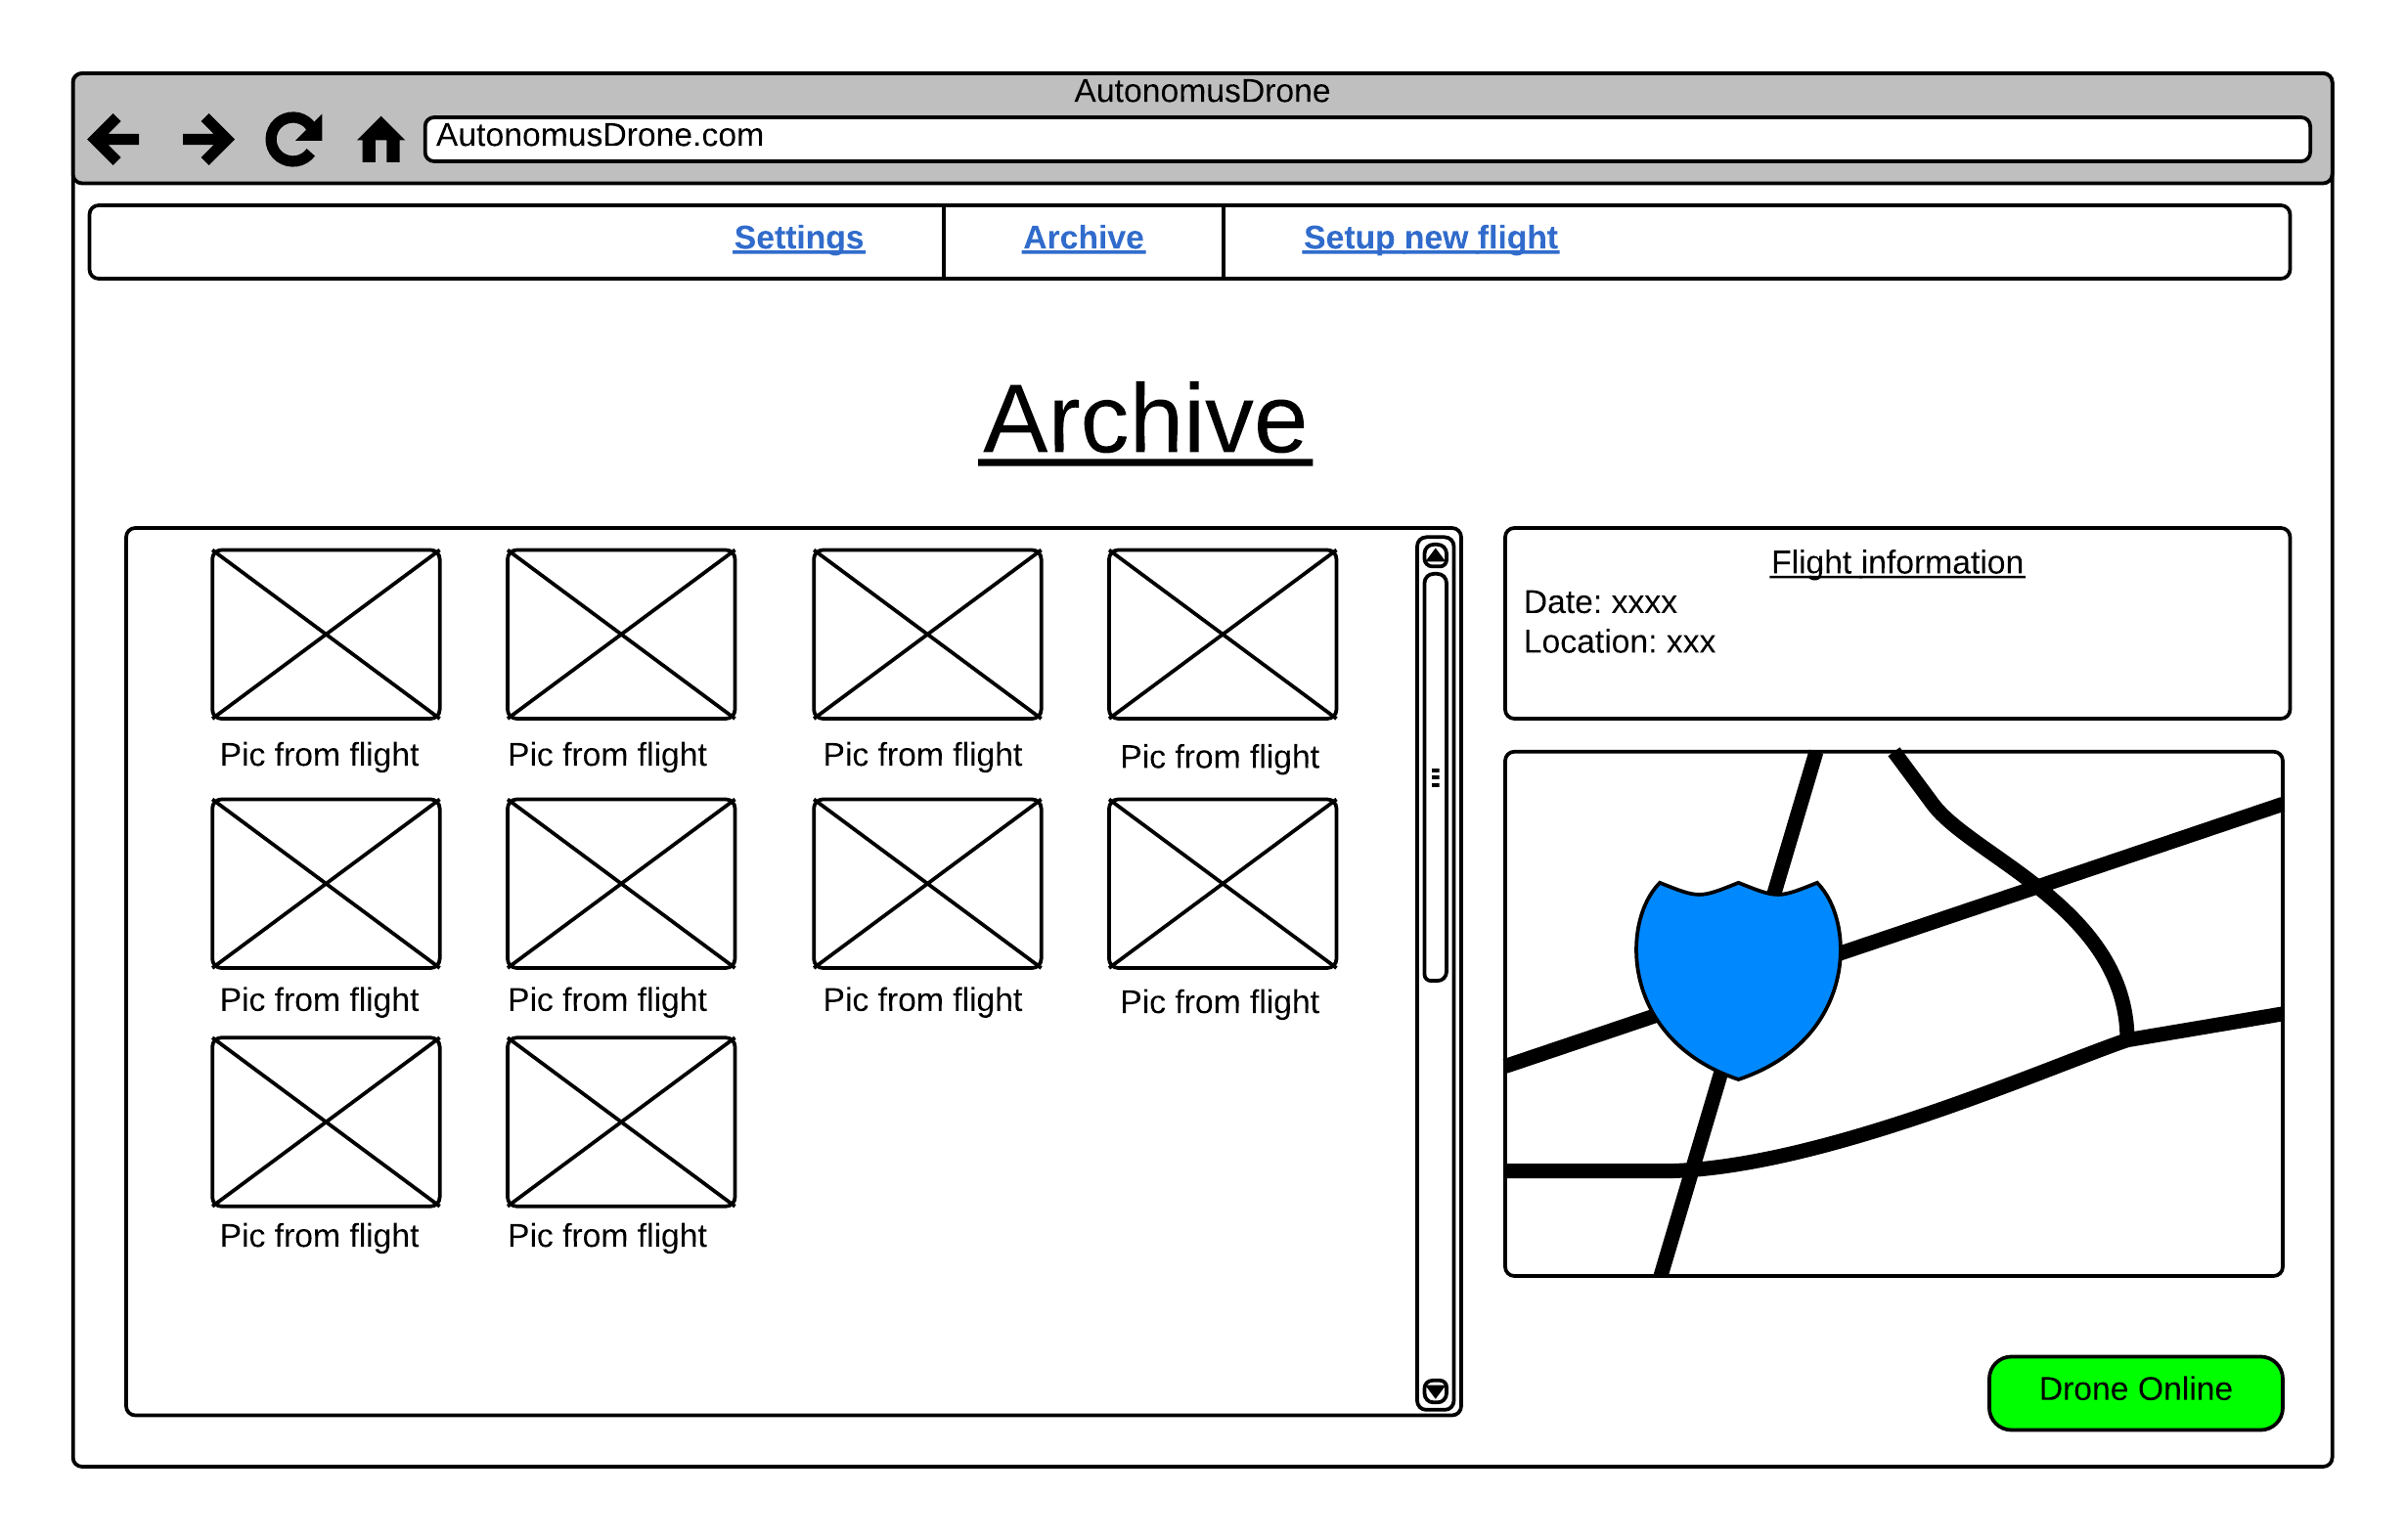
\includegraphics[width=0.9\textwidth]{Billeder/UI_mockups/archive_choosen.png}
	\vspace{-5pt}
	\caption{Tidligere flyverute valgt}
	\label{fig:mockup_archive_choosen}
\end{figure}

\vspace{1cm}

I Opsæt ny flyvning menuen kan bruger indstille ny flyveopsætning. 
Bruger kan indstille sin ønskede flyverute ved at klikke på kortet, og vælge hvilke GPS positioner som dronen skal overvåge og tage billeder af. 
Hver GPS position der vælges præsenteres i tabellen til venstre for kortet. 
I tabellen kan bruger ydermere indstille om der skal tages billeder ved GPS positionerne og hvilken højde dronen skal tage billeder fra. Nedenfor tabellen sættes den generelle flyvehøjde.
Bruger har mulighed for at gemme nylavede flyveopsætninger til senere brug.

\vspace{-5pt}
%Setup new flight mockup
\begin{figure}[H]
	\centering
	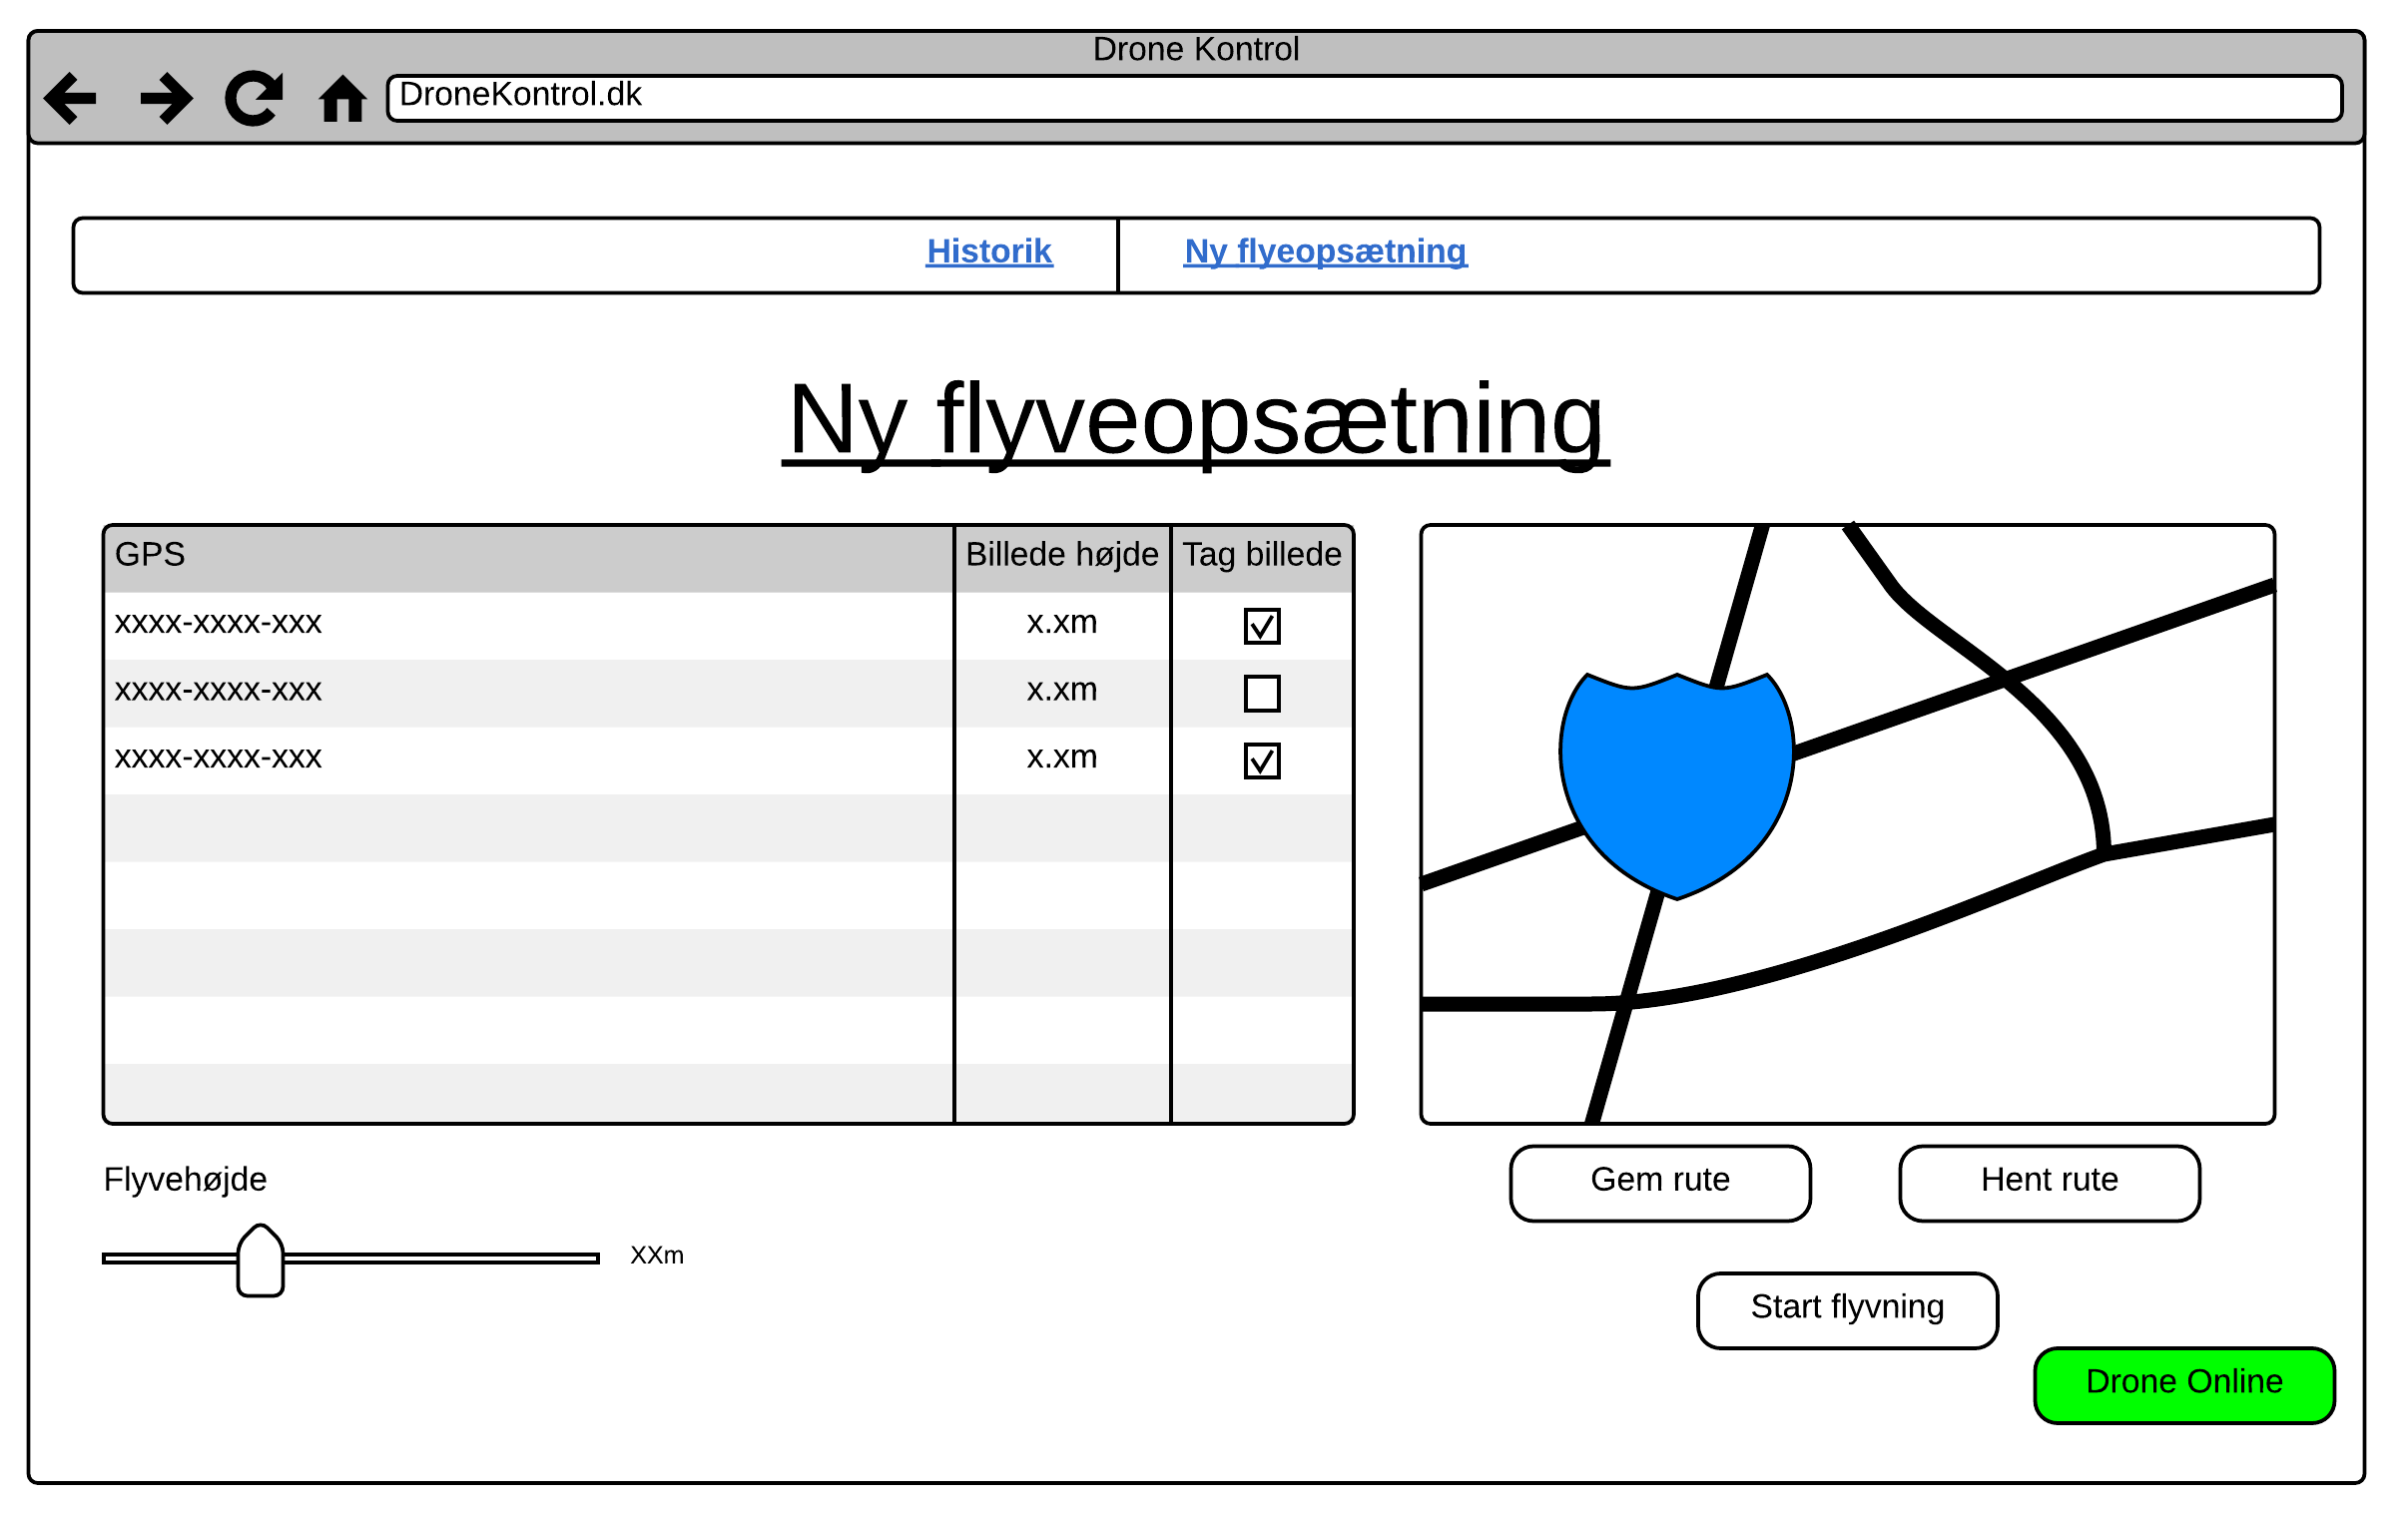
\includegraphics[width=0.9\textwidth]{Billeder/UI_mockups/setup_new_flight.png}
	\vspace{-5pt}
	\caption{Ny flyverute}
	\label{fig:mockup_setup_new_flight}
\end{figure}

 